\chapter{Existující aplikace}\label{chap:ExistingApps}

Existuje několik aplikací, které řeší problém simulace zásobníkových automatů. Některé z nich bych v této kapitole rád popsal.~\cite{Buzatto2023}~\cite{Rodriguez2018}~\cite{Bednarz2023}

% BIB: https://github.com/davidbuzatto/YAAS
\section{YAAS --- Yet Another Automata Simulator}

YAAS --- Yet Another Automata Simulator je aplikace vytvořená profesorem Davidem Buzattem z Instituto Federal de Educação, Ciência e Tecnologia de São Paulo. Tato aplikace obsahuje nejen možnost tvorby zásobníkových automatů, ale i konečných automatů a turingových strojů. Zásobníkové automaty se v aplikaci tvoří graficky --- uživatel si přidá stavy a pak mezi nimi může vytvářet přechody pomocí šipek. Aplikace si z těchto informací sama vytvoří příslušnou vstupní a zásobníkovou abecedu. Při spuštění simulace se pak uživateli zobrazí posloupnost přechodů a zároveň v~grafickém zobrazení obarvuje konkrétní stav, ve kterém se zrovna zásobníkový automat nachází, Obrázek~\ref{fig:YAAS}.

% BIB: https://github.com/DauteRR/PushdownAutomaton
\section{DauteRR --- Pushdown Automaton}

Pushdown automaton od Dauta Rodríguez Rodrígueze je konzolová aplikace napsaná v jazyce Java. Tato aplikace na vstup bere soubor s definicí zásobníkového automatu. Vstupy jsou zadány buď v~druhém vstupním souboru nebo jsou čteny z příkazového řádku. Program dále umožňuje zapnout tzv.~trace mód, který ve výpisu ukazuje jednotlivé kroky a pomocí $>$ označuje, který symbol je zrovna čtený.

\section{Bakalářská práce z roku 2022/2023}

Ve školním roce 2022/2023 byla vytvořena bakalářská práce na stejné téma studentem Danielem Bednarzem. Jedná se o desktopovou aplikaci napsanou v jazyce Python. Aplikace umožňuje vytvářet zásobníkové automaty pomocí formuláře přímo v aplikaci nebo automat nahrát ze souboru. Simulace probíhá graficky, kdy uživatel vidí na rozdíl od aplikace YAAS vstupní pásku, řídící jednotku a~zásobník, Obrázek~\ref{fig:BP}.

\begin{figure}[h]
    \centering
    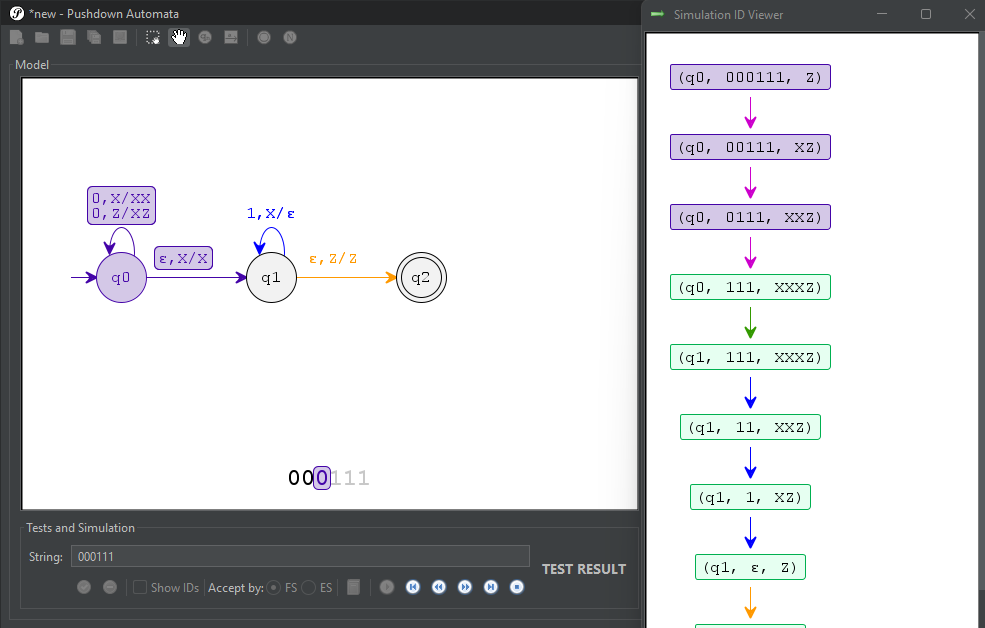
\includegraphics[width=0.6\textwidth]{Figures/PrntScrn_YAAS.png}
    \caption{YAAS v průběhu simulace.}\label{fig:YAAS}
\end{figure}

\begin{figure}[h]
    \centering
    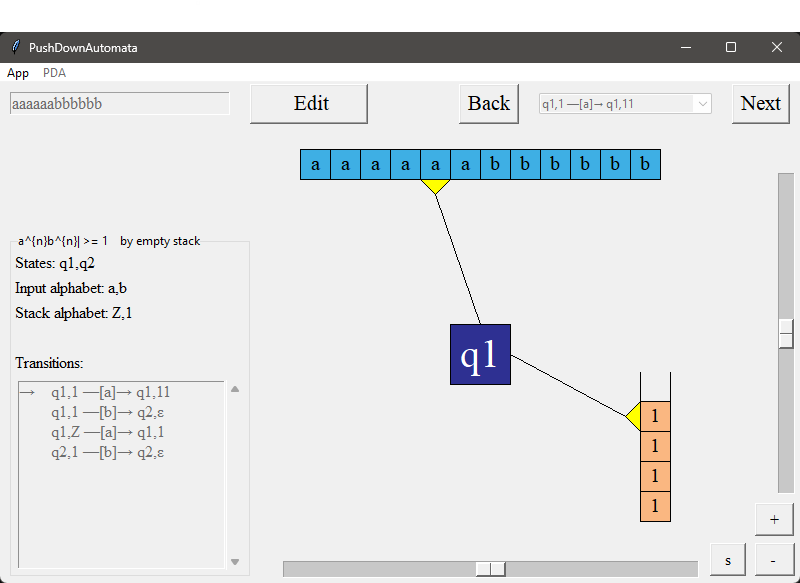
\includegraphics[width=0.55\textwidth]{Figures/PrntScrn_BP.png}
    \caption{Bakalářská práce z roku 2022/2023}\label{fig:BP}
\end{figure}

\section{Shrnutí}

Jak lze vidět výše, existují aplikace, které řeší simulaci zásobníkových automatů různým způsobem. Jeden ze způsobů je výpis do konzole. Další způsoby jsou pak již grafické, kde se objevují dva různé přístupy. Jeden je graf se stavy jako kolečka a přechody znázorněnými jako šipky mezi jednotlivými stavy. Druhý pak zobrazuje komponenty podobně, jako jsou zakresleny na Obrázku~\ref{fig:PDAComponents}.

\endinput